Para el plan de pruebas se construyeron dos opciones para la transmisión de energía con las antenas. Por un lado, el CAERCEM del itba posee un transmisor en la banda UHF de hasta 20W que podríamos utilizar para transmitir. Por otro lado, y mas pegado a la realidad, se utilizará un modulo oscilador en 915MHz en cascada con un amplificador de potencia apto para radiofrecuencia que será alimentado mediante una etapa DC-DC conectado a la batería de la unidad de energía. La salida del amplificador será llevada hasta la antena transmisora utilizando cable mallado RG-58 apto para radiofrecuencia.

\begin{figure}[H]
	\centering
	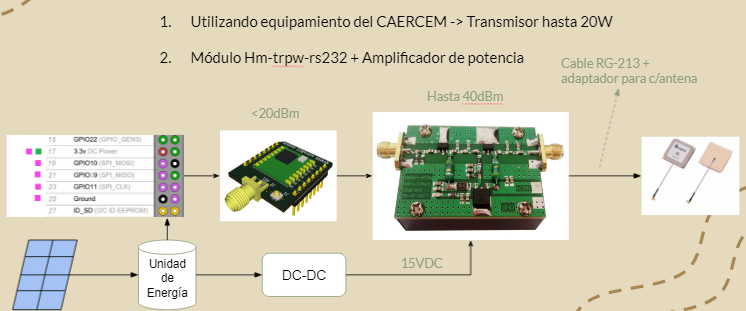
\includegraphics[width=0.8\linewidth]{ImagenesIngenieria de Detalle/planDePruebasAntenasA}	
	\caption{Plan de pruebas Antenas A.}
	\label{fig:planDePruebasAntenasA}
\end{figure}

Del lado de la recepción, se conectará la antena receptora a la placa de evaluación del P1110B y se medirá la tensión en el supercapacitor provisto en esta.


\begin{figure}[H]
	\centering
	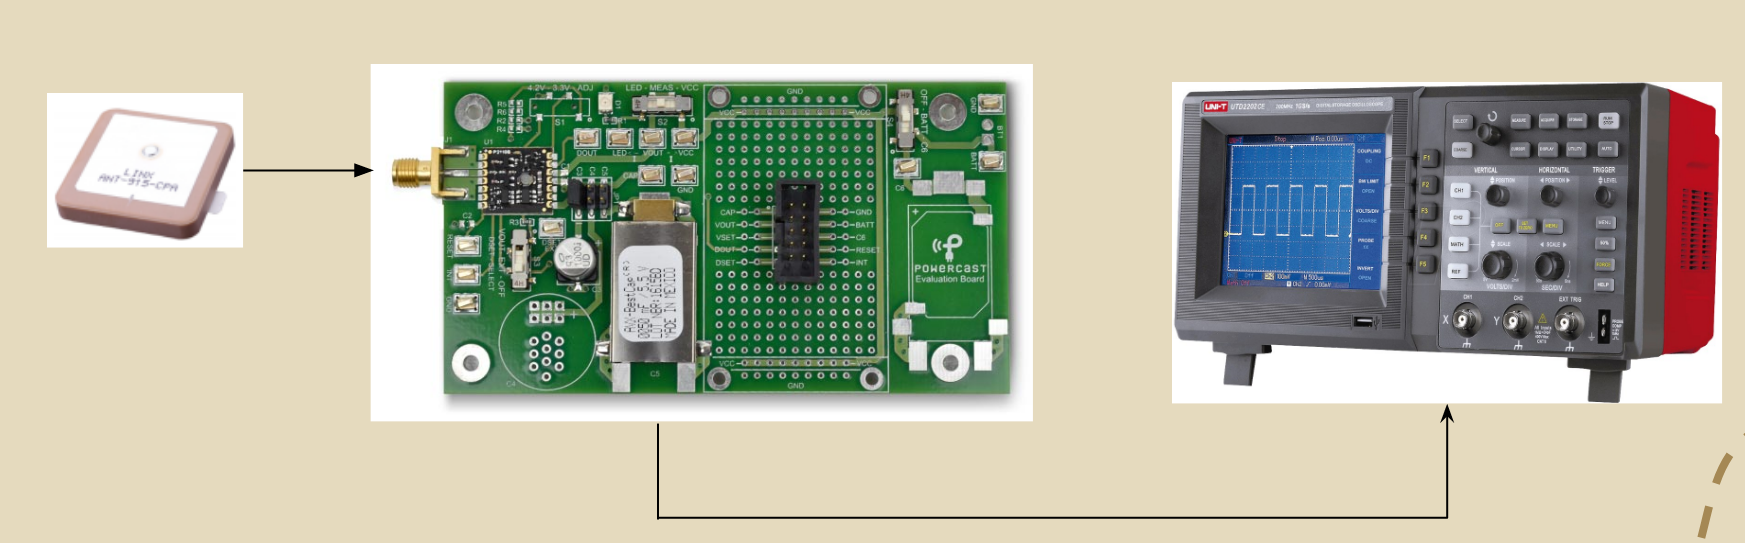
\includegraphics[width=0.8\linewidth]{ImagenesIngenieria de Detalle/planDePruebasAntenasB}	
	\caption{Plan de pruebas Antenas B.}
	\label{fig:planDePruebasAntenasB}
\end{figure}

En cuanto a los sensores se comparan los resultados de los sensores del sistema contra unos previamente calibrados.

\begin{figure}[H]
	\centering
	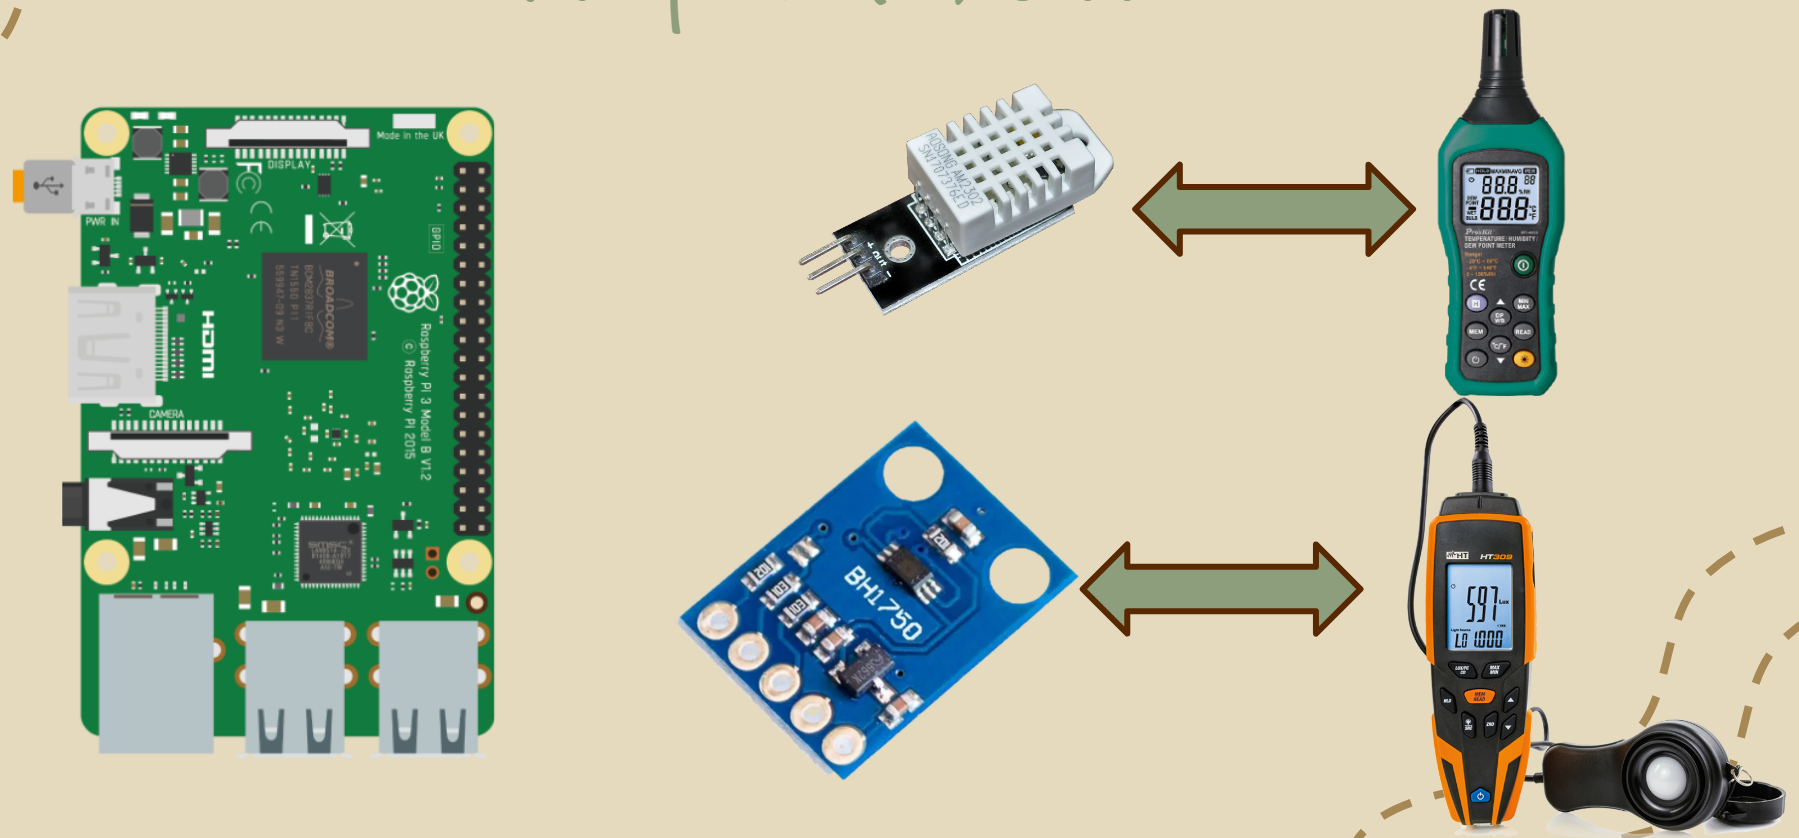
\includegraphics[width=0.8\linewidth]{ImagenesIngenieria de Detalle/planDePruebasSensores}	
	\caption{Plan de pruebas sensores.}
	\label{fig:planDePruebasSensores}
\end{figure}